\documentclass[11pt,a4paper]{article}

\usepackage[margin=2.5cm]{geometry}
\usepackage[utf8]{inputenc}
\usepackage[spanish]{babel}
\usepackage{graphicx}
\usepackage{amsmath}
\usepackage{hyperref}
\usepackage{booktabs}
\usepackage{enumitem}
\usepackage{titlesec}
\usepackage{caption}
\usepackage{subcaption}
\usepackage{float}

\titleformat{\section}{\large\bfseries}{\thesection}{1em}{}
\titleformat{\subsection}{\normalsize\bfseries}{\thesubsection}{1em}{}

\title{Métodos Basados en el Conocimiento Aplicado a Empresas (CAE)\\
       Módulo de Ranking}

\author{
Estudiante: Juan Camilo España Lopera\\
Profesor: Jose Ramón Quevedo Pérez\\[6pt]
Universidad de Oviedo
}

\date{\today}

% ─────────────────────────────────────────────────────────────────────────────
\begin{document}
\maketitle


% =============================================================================
\section{Contexto y motivación}
% =============================================================================

La misma empresa consultora de IA del módulo de cuantificación necesita ahora
\textbf{ordenar} las recomendaciones médicas de un LLM de mejor a peor, según
la preferencia de los expertos. Este orden permite presentar primero las
recomendaciones más fiables y detectar patrones en las peor valoradas.

Para obtener estas preferencias, grupos de expertos evaluaron lotes de
recomendaciones asignando una calificación de 0 a 10 a cada una. Con esas
calificaciones se entrena un modelo que aprende a ordenar nuevas
recomendaciones automáticamente, sin necesidad de seguir contratando expertos.

Cada recomendación está descrita por los mismos 10 atributos de texto del
módulo anterior (\texttt{n\_words}, \texttt{n\_refs}, \texttt{lex\_div},
\texttt{hedge\_r}, \texttt{spec\_sc}, \texttt{sent\_pol}, \texttt{consist},
\texttt{src\_dens}, \texttt{num\_dens}, \texttt{verb\_ten}).

\begin{table}[H]
\centering
\caption{Conjuntos de datos de ranking disponibles}
\begin{tabular}{lcccl}
\toprule
\textbf{Dataset} & \textbf{Recomendaciones únicas} & \textbf{Lotes (expertos)} & \textbf{Filas totales} & \textbf{Rol} \\
\midrule
ranking\_E1 & 418 & 200 & 1\,000 & Train/Test \\
ranking\_E2 & 255 & 100 &   500  & Train/Test \\
dataset\_E3 & 313 &  -- &   313  & Producción \\
\bottomrule
\end{tabular}
\end{table}

Las recomendaciones de E1 y E2 son las mismas del módulo de cuantificación
(mismos atributos, sin la columna \texttt{y\_alucinacion}). Cada experto
evalúa 5 recomendaciones distintas seleccionadas del dataset, por lo que una
misma recomendación puede aparecer en varios lotes con distintas calificaciones, compitiendo con recomendaciones diferentes.


% =============================================================================
\section{Definición del problema}
% =============================================================================

El problema es de \textbf{ranking por lotes}: dado un lote de $k$
recomendaciones evaluadas con calificaciones $c_1, \ldots, c_k \in [0,10]$,
se quiere aprender un modelo que asigne puntuaciones $\hat{s}_i$ tales que
el orden de las puntuaciones coincida con el de las calificaciones reales:

\begin{equation}
    c_i > c_j \;\Rightarrow\; \hat{s}_i > \hat{s}_j
\end{equation}

La dificultad es que las calificaciones son \textbf{locales a cada lote}
(cada experto usa su propia escala), pero el modelo debe producir un
\textbf{ranking global} aplicable a las 313 recomendaciones de E3.


% =============================================================================
\section{Preprocesamiento}
% =============================================================================

Cada fila de los datasets de ranking tiene la estructura
\texttt{[calificacion, lote, atrib\_1, \ldots, atrib\_10]}:

\begin{itemize}
    \item $Y$: columnas \texttt{calificacion} y \texttt{lote} — etiqueta de
    preferencia e identificador del lote al que pertenece cada recomendación.
    \item $X$: las 10 columnas de atributos de texto.
\end{itemize}

E1 y E2 se concatenan en un único conjunto de entrenamiento (1\,500 filas
en total: 1\,000 de E1 + 500 de E2) para aprovechar todas las preferencias
disponibles. Cada fila es una evaluación de una recomendación por un experto.

La validación cruzada usa \texttt{GroupKFold} con grupos definidos por el
identificador de lote, de modo que las recomendaciones de un mismo lote
nunca se dividen entre entrenamiento y test.

\begin{figure}[H]
    \centering
    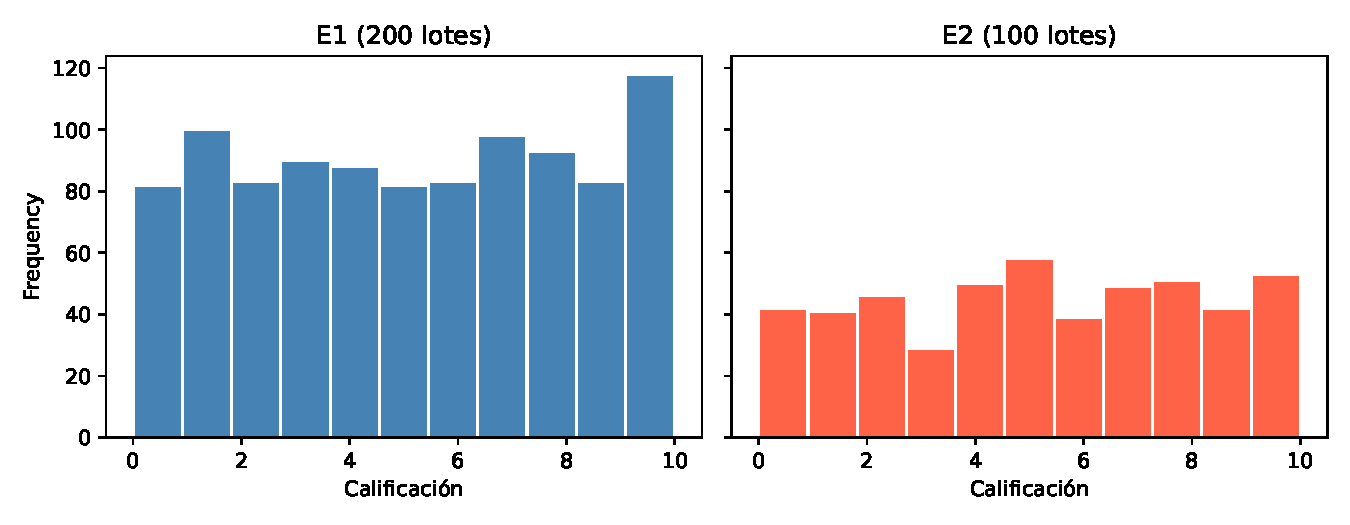
\includegraphics[width=0.85\textwidth]{figures/hist_calificaciones.pdf}
    \caption{Distribución de las calificaciones asignadas por los expertos
             en E1 (azul) y E2 (rojo). Ambos siguen una distribución similar
             y uniforme entre 0 y 10, sin sesgo visible hacia un extremo.}
    \label{fig:calificaciones}
\end{figure}


% =============================================================================
\section{Métodos de ranking}
% =============================================================================

Se comparan tres modelos, todos entrenados sobre el conjunto combinado
E1\,+\,E2:

\subsection*{linearRank}
Modelo lineal basado en SVM. Para cada par de recomendaciones del mismo lote
con calificaciones distintas, genera un ejemplo de comparación cuya etiqueta
indica cuál de las dos es preferida. El modelo aprende qué recomendación es
mejor a partir de la diferencia de sus atributos. Es sencillo e interpretable,
pero solo captura relaciones lineales.

\subsection*{XGBRanker pairwise}
Modelo de gradient boosting (XGBoost) que minimiza el número de pares mal
ordenados dentro de cada lote (\texttt{rank:pairwise}). Captura relaciones
no lineales entre atributos.

\subsection*{XGBRanker ndcg}
Igual que el anterior pero optimiza directamente el NDCG, métrica que
penaliza más los errores en las primeras posiciones del ranking
(\texttt{rank:ndcg}).


% =============================================================================
\section{Selección de modelos}
% =============================================================================

Los tres modelos se evalúan con \textbf{validación cruzada de 3 folds}
(\texttt{GroupKFold} por lote) sobre E1+E2. Las métricas son:

\begin{itemize}
    \item \textbf{C-index:} fracción de pares correctamente ordenados dentro
    de cada lote (0.5\,=\,azar, 1.0\,=\,perfecto).
    \item \textbf{NDCG:} calidad del ranking ponderando más los errores en
    las primeras posiciones (0\,=\,peor, 1\,=\,perfecto).
\end{itemize}

\begin{figure}[H]
    \centering
    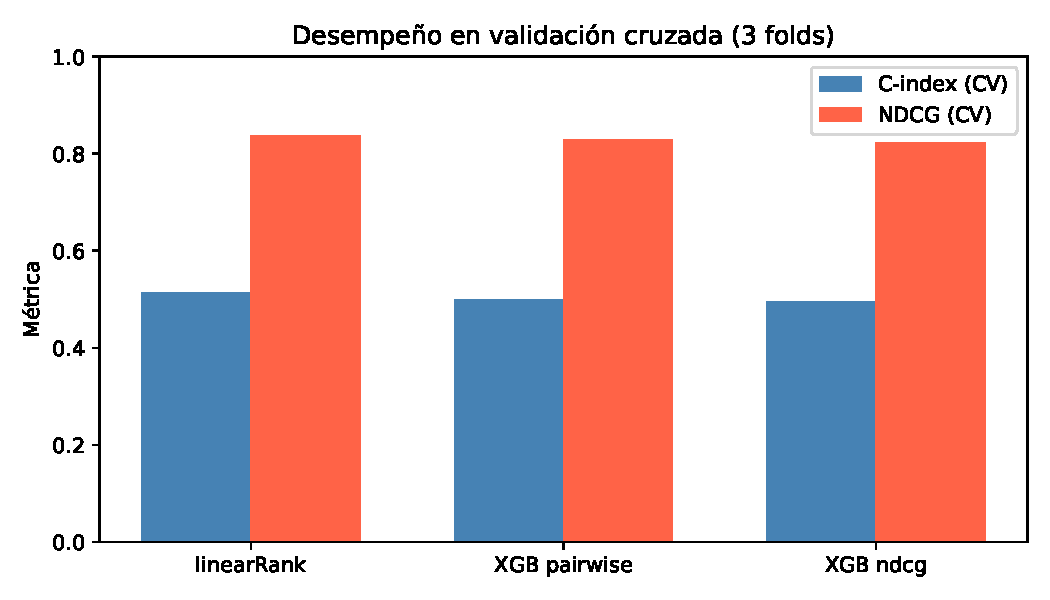
\includegraphics[width=0.72\textwidth]{figures/cv_metricas.pdf}
    \caption{C-index y NDCG en validación cruzada (3 folds) para los tres
             modelos. Las barras muestran el promedio sobre los 3 folds.}
    \label{fig:cv_metricas}
\end{figure}


% =============================================================================
\section{Metodología experimental}
% =============================================================================

La evaluación sigue dos pasos:

\begin{enumerate}
    \item \textbf{Métrica en entrenamiento.} Cada modelo se entrena y evalúa
    sobre el mismo conjunto completo E1+E2. Un C-index alto aquí pero bajo
    en validación cruzada indica sobreajuste.

    \item \textbf{Validación cruzada por lotes.} Se aplica \texttt{GroupKFold}
    con 3 folds, garantizando que las recomendaciones de un mismo lote queden
    siempre en el mismo fold. Se reporta el promedio de C-index y NDCG.
\end{enumerate}

El mejor modelo es el que maximiza ambas métricas en validación cruzada.


% =============================================================================
\section{Evaluación de resultados}
% =============================================================================

\subsection{Sobreajuste vs.\ generalización}

\begin{table}[H]
\centering
\caption{C-index y NDCG en entrenamiento y en validación cruzada (3 folds)}
\begin{tabular}{lcccc}
\toprule
 & \multicolumn{2}{c}{\textbf{Entrenamiento}} & \multicolumn{2}{c}{\textbf{CV (3 folds)}} \\
\cmidrule(lr){2-3}\cmidrule(lr){4-5}
\textbf{Modelo} & C-index & NDCG & C-index & NDCG \\
\midrule
linearRank         & 0.5071 & 0.8281 & 0.5149 & 0.8367 \\
XGBRanker pairwise & 0.8210 & 0.9484 & 0.5003 & 0.8292 \\
XGBRanker ndcg     & 0.7396 & 0.9474 & 0.4957 & 0.8242 \\
\bottomrule
\end{tabular}
\end{table}

Los modelos XGBoost muestran un sobreajuste claro: su C-index en entrenamiento
es muy alto (0.82 y 0.74) pero cae a valores cercanos al azar (0.50) en
validación cruzada. El NDCG se mantiene estable en todos los casos porque
esta métrica pondera más los errores en las primeras posiciones y es menos
sensible a errores en el resto del ranking.

\subsection{Selección del mejor modelo}

El modelo seleccionado fue \textbf{linearRank}, ya que fue el único que mostró resultados coherentes entre el entrenamiento y la validación cruzada (C-index$\approx$0.51 en ambos casos). Aunque su C-index absoluto es moderado, presenta las mejores métricas de validación cruzada y, por lo tanto, es el que mejor capacidad de generalización muestra frente a nuevos lotes.

% =============================================================================
\section{Paso a producción}
% =============================================================================

El modelo linearRank se aplica sobre las 313 recomendaciones de E3, que son
las mismas del módulo de cuantificación sin etiquetas de alucinación. Para
cada recomendación se calcula una puntuación; las
recomendaciones se ordenan de mayor a menor puntuación y se les asigna
una posición global (\texttt{rank\_predicho}).

Las puntuaciones oscilan entre $-3.27$ y $3.91$. Una distribución amplia
indica que el modelo diferencia bien entre recomendaciones.

\begin{figure}[H]
    \centering
    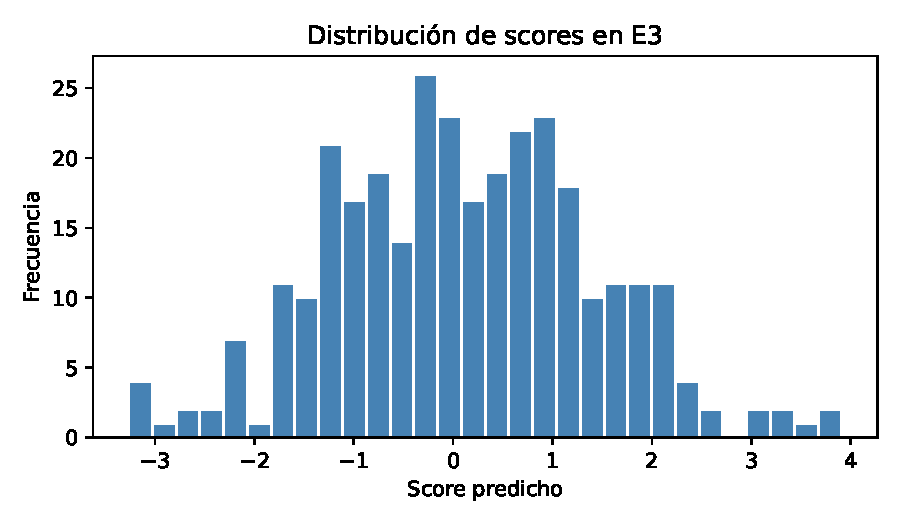
\includegraphics[width=0.60\textwidth]{figures/scores_E3.pdf}
    \caption{Distribución de las puntuaciones asignadas a las 313
             recomendaciones de E3. La separación entre scores positivos
             y negativos refleja la capacidad del modelo para distinguir
             recomendaciones preferidas de las no preferidas.}
    \label{fig:scores_e3}
\end{figure}

Las cinco recomendaciones mejor valoradas por el modelo son:

\begin{table}[H]
\centering
\caption{Top-5 recomendaciones de E3 según el ranking predicho}
\begin{tabular}{ccc}
\toprule
\textbf{id} & \textbf{rank\_predicho} & \textbf{score\_predicho} \\
\midrule
14  & 1 & 3.9123 \\
118 & 2 & 3.7413 \\
300 & 3 & 3.4818 \\
28  & 4 & 3.3677 \\
142 & 5 & 3.2144 \\
\bottomrule
\end{tabular}
\end{table}


% =============================================================================
\section{Conclusiones}
% =============================================================================

\begin{itemize}
    \item \textbf{C-index bajo en todos los modelos:} Los valores de C-index
    en validación cruzada son cercanos al azar (0.50) para los tres modelos.
    Esto es razonable dado que las calificaciones de los expertos se generaron
    aleatoriamente, por lo que no existe un patrón real en las preferencias
    que los modelos puedan aprender. Para obtener C-index significativamente
    mayor que 0.5 sería necesario que las calificaciones siguieran un modelo
    basado en los atributos de las recomendaciones.

    \item \textbf{XGBoost sobreajusta:} Ambos modelos XGBoost obtienen un
    C-index alto en entrenamiento (0.82 y 0.74) pero caen al nivel del azar
    en validación cruzada (0.50), lo que indica que memorizan los lotes de
    entrenamiento sin aprender patrones generalizables.

    \item \textbf{linearRank es el más fiable:} Mantiene un C-index estable
    entre entrenamiento (0.51) y validación cruzada (0.51), sin sobreajuste.
    Su simplicidad resulta una ventaja cuando los lotes son pequeños
    (5 recomendaciones por lote) y las preferencias son ruidosas.

    \item \textbf{El NDCG es menos discriminante:} Los tres modelos obtienen
    valores similares en validación cruzada (0.82--0.84), lo que sugiere que
    todos ordenan bien las primeras posiciones aunque difieran en el resto.

    \item \textbf{Resultado en producción:} linearRank produce un ranking
    global de las 313 recomendaciones de E3 con scores entre $-3.27$ y
    $3.91$, permitiendo priorizar las recomendaciones más fiables sin
    necesidad de revisión manual por expertos.
\end{itemize}

\end{document}
